\documentclass[10pt,a4paper]{article}
\usepackage[a4paper,margin=2.1cm]{geometry}
\usepackage{amsmath,amssymb}
\usepackage{booktabs,array}
\usepackage{graphicx}
\usepackage{enumitem}
\usepackage[siunitx]{circuitikz}
\usepackage{xcolor}
\usepackage[hidelinks]{hyperref}
\usepackage{caption}
\usepackage{float}
\captionsetup{font=small,labelfont=bf}
\setlist{itemsep=0.2ex,topsep=0.4ex}
\usepackage[htt]{hyphenat}
\emergencystretch=3em
\newcommand{\VOUT}{V_{OUT}}
\newcommand{\VIN}{V_{IN}}
\newcommand{\IL}{I_{L}}

\title{A 1.5\,V, 50\,mA PMOS LDO in SkyWater sky130:\\ schematic, layout and sign-off with the open PDK decks}
\author{Vu-Quoc-Minh Nguyen}
\date{09 November 2026}

\begin{document}
\maketitle

\begin{abstract}
\noindent A low-dropout regulator ($\VIN = 1.8$\,V, $\VOUT = 1.5$\,V, $\IL$ up to 50\,mA, $C_L = 2.2\,\mu$F) is designed in SkyWater sky130 with the 1.8\,V devices, laid out in Electric by a script, and checked with the official open-source decks of the PDK: KLayout DRC (\texttt{sky130A\_mr.drc}: 0 violations) and KLayout LVS (\texttt{sky130.lvs}: netlists match, including the poly resistors). Current densities are checked against the limits of the SkyWater technology LEF; the first layout failed them and the power routing was redone. Parasitics are extracted with KLayout-PEX (2.5D engine, RC) and the performance is simulated again on the extracted netlist. All numbers in this report are produced by the scripts of the repository.
\end{abstract}

\section{Specification and result summary}

\begin{table}[H]
\centering\small
\caption{Schematic (typical corner, 27\,\textdegree C) against post-layout (extracted RC netlist). $^\dagger$: the phase does not reach $-180^\circ$ below 1\,GHz. Schematic DC sweeps: 0.1\,mA / 2\,mV steps; post-layout: 0.5\,mA / 10\,mV steps.}
\label{tab:summary}
\begin{tabular}{lccc}
\toprule
quantity & target & schematic & post-layout \\
\midrule
$\VOUT$ at $\IL = 0.1$\,mA (V) & 1.5 & 1.5006 & 1.5008 \\
$\VOUT$ at $\IL = 50$\,mA (V) &  & 1.4959 & 1.4948 \\
load regulation 0.1$\to$50\,mA (mV) &  & 4.73 & 6.08 \\
line regulation 1.7--1.9\,V, 0.1\,mA (mV/V) &  & 14.2 & 16.5 \\
line regulation 1.7--1.9\,V, 50\,mA (mV/V) &  & 23.0 & 25.1 \\
dropout ($\VOUT$ $-1\%$) at 50\,mA (mV) &  & 142 & 170 \\
quiescent current at 1.8\,V ($\mu$A) &  & 64.7 & 64.3 \\
PSRR at 1\,kHz, 0.1\,mA (dB) &  & 35.6 & 36.0 \\
PSRR at 1\,kHz, 50\,mA (dB) &  & 33.6 & 33.2 \\
phase margin, 0.1\,mA (\textdegree) & $\ge 45$ & 89.0 & 89.7 \\
phase margin, 1\,mA (\textdegree) &  & 89.5 & 91.6 \\
phase margin, 10\,mA (\textdegree) &  & 85.9 & 98.6 \\
phase margin, 50\,mA (\textdegree) &  & 80.2 & 101.6 \\
unity-gain frequency, 0.1\,mA (kHz) &  & 43 & 43 \\
unity-gain frequency, 50\,mA (kHz) &  & 1519 & 1369 \\
gain margin, 0.1\,mA (dB) & & 74 & none$^\dagger$ \\
gain margin, 50\,mA (dB) & & 56 & none$^\dagger$ \\
load step: dip below the 0.1\,mA level (mV) &  & 4.64 & 6.01 \\
load step: peak above the 50\,mA level (mV) &  & 4.62 & 6.01 \\
\bottomrule
\end{tabular}
\end{table}

\noindent Process corners (schematic): tt, ss, ff, sf, fs, ll, hh $\times$ $-40$, 27, 125\,\textdegree C $\times$ $\VIN = 1.7, 1.8, 1.9$\,V (63 cases): $\VOUT$ = 1.4922--1.5202\,V at 0.1\,mA and 1.4877--1.5003\,V at 50\,mA, quiescent current 63.4--66.7\,$\mu$A, lowest phase margin 75.6\textdegree\ (ss, -40\,\textdegree C, $\VIN$ = 1.9\,V).

\section{Circuit}

\begin{figure}[H]
\centering
% sky130 LDO schematic (circuitikz); \input by ldo_sky130.tex
\begin{circuitikz}[scale=0.88, transform shape, american]
  \def\VIN{6.4}
  % ------------------------------------------------ rails
  \draw (-0.6,\VIN) -- (14.2,\VIN) node[right] {$V_{IN}$};
  \draw (-0.6,0) -- (14.2,0);
  \node[ground] at (7.0,0) {};

  % ------------------------------------------------ bias: I_BIAS into the NMOS diode MBN, mirrored to MT
  \draw (0,\VIN) to[american current source, l_={$I_{BIAS}$}] (0,2.4);
  \node[nmos, xscale=-1] (mbn) at (0,1.1) {};
  \node[left] at (-0.2,0.85) {\scriptsize $M_{BN}$};
  \draw (0,2.4) -- (mbn.D);
  \draw (mbn.S) -- (0,0);
  \draw (0,2.05) node[circ] {} -| (0.9,1.1);
  \draw (mbn.G) -- (2.1,1.1);
  \node[nmos] (mt) at (2.6,1.1) {};
  \node[right] at (2.7,0.85) {\scriptsize $M_T$};
  \draw (mt.S) -- (2.6,0);
  \draw (mt.D) -- (2.6,2.2);

  % ------------------------------------------------ NMOS input pair: M1 gate = V_REF (left), M2 gate = V_FB (right)
  \draw (1.8,2.2) -- (3.4,2.2);
  \node[nmos] (m1) at (1.8,3.0) {};
  \node[nmos, xscale=-1] (m2) at (3.4,3.0) {};
  \draw (m1.S) -- (1.8,2.2);
  \draw (m2.S) -- (3.4,2.2);
  \node[right] at (1.85,3.35) {\scriptsize $M_1$};
  \node[left] at (3.35,3.35) {\scriptsize $M_2$};
  \draw (m1.G) -- ++(-0.1,0) node[left] {\scriptsize $V_{REF}$};
  \draw (m2.G) -- ++(0.1,0) node[right] {\scriptsize $V_{FB}$};

  % ------------------------------------------------ PMOS mirror load: M3 (diode), M4
  \node[pmos, xscale=-1] (m3) at (1.8,5.3) {};
  \node[pmos] (m4) at (3.4,5.3) {};
  \node[left] at (1.7,5.55) {\scriptsize $M_3$};
  \node[right] at (3.5,5.55) {\scriptsize $M_4$};
  \draw (m3.S) -- (1.8,\VIN);
  \draw (m4.S) -- (3.4,\VIN);
  \draw (m1.D) -- (m3.D);
  \draw (m2.D) -- (m4.D);
  \draw (m3.G) -- (m4.G);
  \draw (1.8,4.3) node[circ] {} -| (2.6,5.3) node[circ] {};
  \node[left] at (1.8,4.3) {\scriptsize $d_1$};
  \draw (3.4,4.15) node[circ] {} -- (4.6,4.15) |- (5.0,1.1);
  \node[above] at (4.1,4.15) {\scriptsize $V_{EA}$};

  % ------------------------------------------------ gate driver: MCS (common source), MD (diode, 1:N with MP), MBL (bleeder)
  \node[nmos] (mcs) at (5.5,1.1) {};
  \node[right] at (5.6,0.85) {\scriptsize $M_{CS}$};
  \draw (mcs.S) -- (5.5,0);
  \draw (mcs.D) -- (5.5,4.1);
  \node[pmos, xscale=-1] (md) at (5.5,5.3) {};
  \node[left] at (5.4,5.55) {\scriptsize $M_D$};
  \draw (md.S) -- (5.5,\VIN);
  \draw (md.D) -- (5.5,4.1) node[circ] {};
  \draw (md.G) -- ++(0.3,0) coordinate (mdg) -- (mdg |- 0,4.1) node[circ] {};
  \node[pmos] (mbl) at (7.3,5.3) {};
  \node[right] at (7.4,5.55) {\scriptsize $M_{BL}$};
  \draw (mbl.S) -- (7.3,\VIN);
  \draw (mbl.D) -- (7.3,4.1);
  \draw (2.6,5.3) -- (2.6,5.95) -- (6.6,5.95) |- (mbl.G);
  \draw (5.5,4.1) -- (8.6,4.1);
  \node[below] at (6.6,4.1) {\scriptsize $V_G$};

  % ------------------------------------------------ pass device MP
  \node[pmos] (mp) at (9.1,5.3) {};
  \node[right] at (9.2,5.55) {\scriptsize $M_P$};
  \draw (mp.S) -- (9.1,\VIN);
  \draw (8.6,4.1) |- (mp.G);
  \draw (mp.D) -- (9.1,3.75) node[circ] {} -- (14.0,3.75) node[right] {$V_{OUT}$};

  % ------------------------------------------------ divider R1 / R2 (xhigh_po units)
  \draw (10.4,3.75) node[circ] {} to[R, l_=$R_1$] (10.4,1.9) node[circ] {}
        to[R, l_=$R_2$] (10.4,0);
  \draw (10.4,1.9) -- (11.0,1.9) node[right] {\scriptsize $V_{FB}$};

  % ------------------------------------------------ off chip: CL + ESR, IL
  \draw (12.2,3.75) node[circ] {} to[C, l_=$C_L$] (12.2,1.9) to[R, l_=$R_{ESR}$] (12.2,0);
  \draw (13.5,3.75) node[circ] {} to[american current source, l_=$I_L$] (13.5,0);
\end{circuitikz}

\caption{The LDO. On chip: everything except $V_{REF}$, $I_{BIAS}$, $C_L$, $R_{ESR}$ and $I_L$.}
\label{fig:sch}
\end{figure}

\noindent The error amplifier is a five-transistor OTA with an NMOS input pair ($M_1$: $V_{REF}$, $M_2$: $V_{FB}$) and a PMOS mirror load. Its output $V_{EA}$ drives the common-source NMOS $M_{CS}$, which sinks its current from the diode-connected PMOS $M_D$. $M_D$ and the pass device $M_P$ have the same channel length and finger width, so they form a $1:160$ current mirror and the gate node $V_G$ has the low impedance $1/g_{m,D}$: the pole at the large gate capacitance of $M_P$ moves to high frequency, and the output pole set by $C_L$ dominates. The bleeder $M_{BL}$ (a mirror of $M_3$) supplies a small fixed current into $V_G$, so that the subthreshold leakage of $M_{CS}$ at hot corners, multiplied by the mirror ratio, does not exceed the minimum load. The divider is made of identical \texttt{xhigh\_po} poly resistors ($w = 0.35\,\mu$m, $l = 4.27\,\mu$m each): $R_1$ = 2 units, $R_2$ = 4 units, so $\VOUT = V_{REF}(1 + R_1/R_2) = 1.50$\,V.

\begin{table}[H]
\centering\small
\caption{Device sizes (\texttt{scripts/sizes.json}). $W$ per finger.}
\begin{tabular}{llccc}
\toprule
device & type & $W$ ($\mu$m) & $L$ ($\mu$m) & fingers \\
\midrule
$M_{BN}$ & nfet\_01v8 & 4 & 1 & 1 \\
$M_T$ & nfet\_01v8 & 4 & 1 & 4 \\
$M_1$, $M_2$ & nfet\_01v8 & 8 & 1 & 2 \\
$M_3$, $M_4$ & pfet\_01v8 & 8 & 1 & 2 \\
$M_{CS}$ & nfet\_01v8 & 10 & 0.5 & 2 \\
$M_D$ & pfet\_01v8 & 10 & 0.15 & 1 \\
$M_{BL}$ & pfet\_01v8 & 4 & 1 & 1 \\
$M_P$ & pfet\_01v8 & 10 & 0.15 & 160 \\
$R_1$, $R_2$ units & res\_xhigh\_po\_0p35 & 0.35 & 4.27 & 2 + 4 (+2 dummies) \\
bias, load & -- & \multicolumn{3}{l}{$I_{BIAS}$ = 10\,$\mu$A, $V_{REF}$ = 1\,V, $C_L$ = 2.2\,$\mu$F, $R_{ESR}$ = 10\,m$\Omega$} \\
\bottomrule
\end{tabular}
\end{table}

\section{Layout}

The layout is generated by \texttt{layout/gen\_layout.py} in Electric 9.08 (built-in \texttt{skywater130} technology) and exported to GDS; \texttt{layout/postproc.py} then adds the two things Electric does not write: the \texttt{poly\_rs} marker (66/13) on the resistor bodies, without which the decks see no precision resistor, and the pin labels (70/5). Size $\approx 155.3 \times 40.6\,\mu\mathrm{m}$.

\begin{figure}[H]
\centering
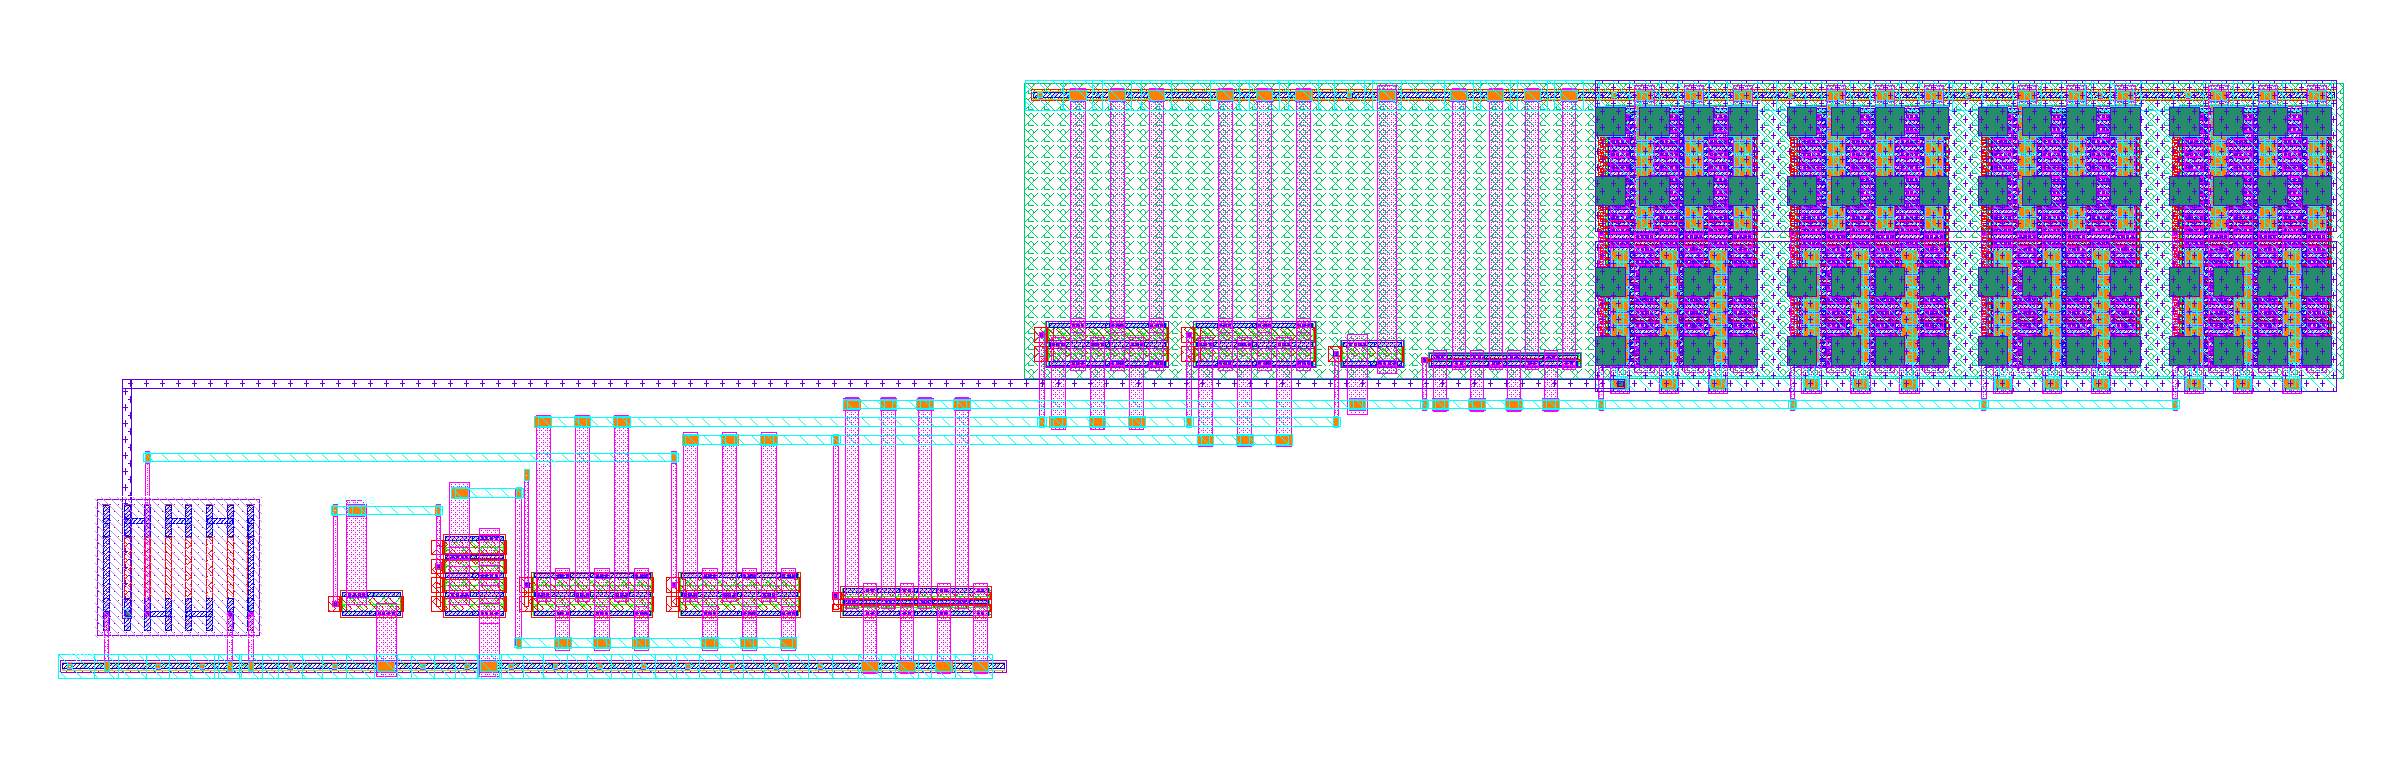
\includegraphics[width=\linewidth]{../figures/layout_full.png}
\caption{\texttt{ldo\_final.gds} (KLayout, sky130 layer colours). Left to right: divider (6 units + 2 dummies), NMOS row ($M_{BN}$, $M_T$, $M_1$, $M_2$, $M_{CS}$) with the met3 signal tracks above it, PMOS row ($M_3$, $M_4$, $M_{BL}$, $M_D$) in the n-well, and the pass device (4 columns $\times$ 40 fingers) under the power plates.}
\label{fig:layout}
\end{figure}

\paragraph{Power path.} The pass device carries the whole load current. Its drain and source rows are joined by vertical met2 straps (three of each per column). In the first layout the straps ended on a met3 rail of 1\,$\mu$m (vout) or 2\,$\mu$m (vin) width, and the vin pin sat 45\,$\mu$m away from the array; 50\,mA in these rails is 50 and 25\,mA/$\mu$m, far above the met3 limit of 6.8\,mA/$\mu$m (Sec.~\ref{sec:em}). The final layout covers the array with two met3 + met4 plates, vout over the lower half and vin over the upper half (about 9.4\,$\mu$m tall each). Every drain (source) row inside the vout (vin) plate has a via2 of $3\times2$ cuts from its strap, the two plate layers are joined by 800 / 801 via3 cuts each, and the vin and vout pins are at the plate centres.

\begin{figure}[H]
\centering
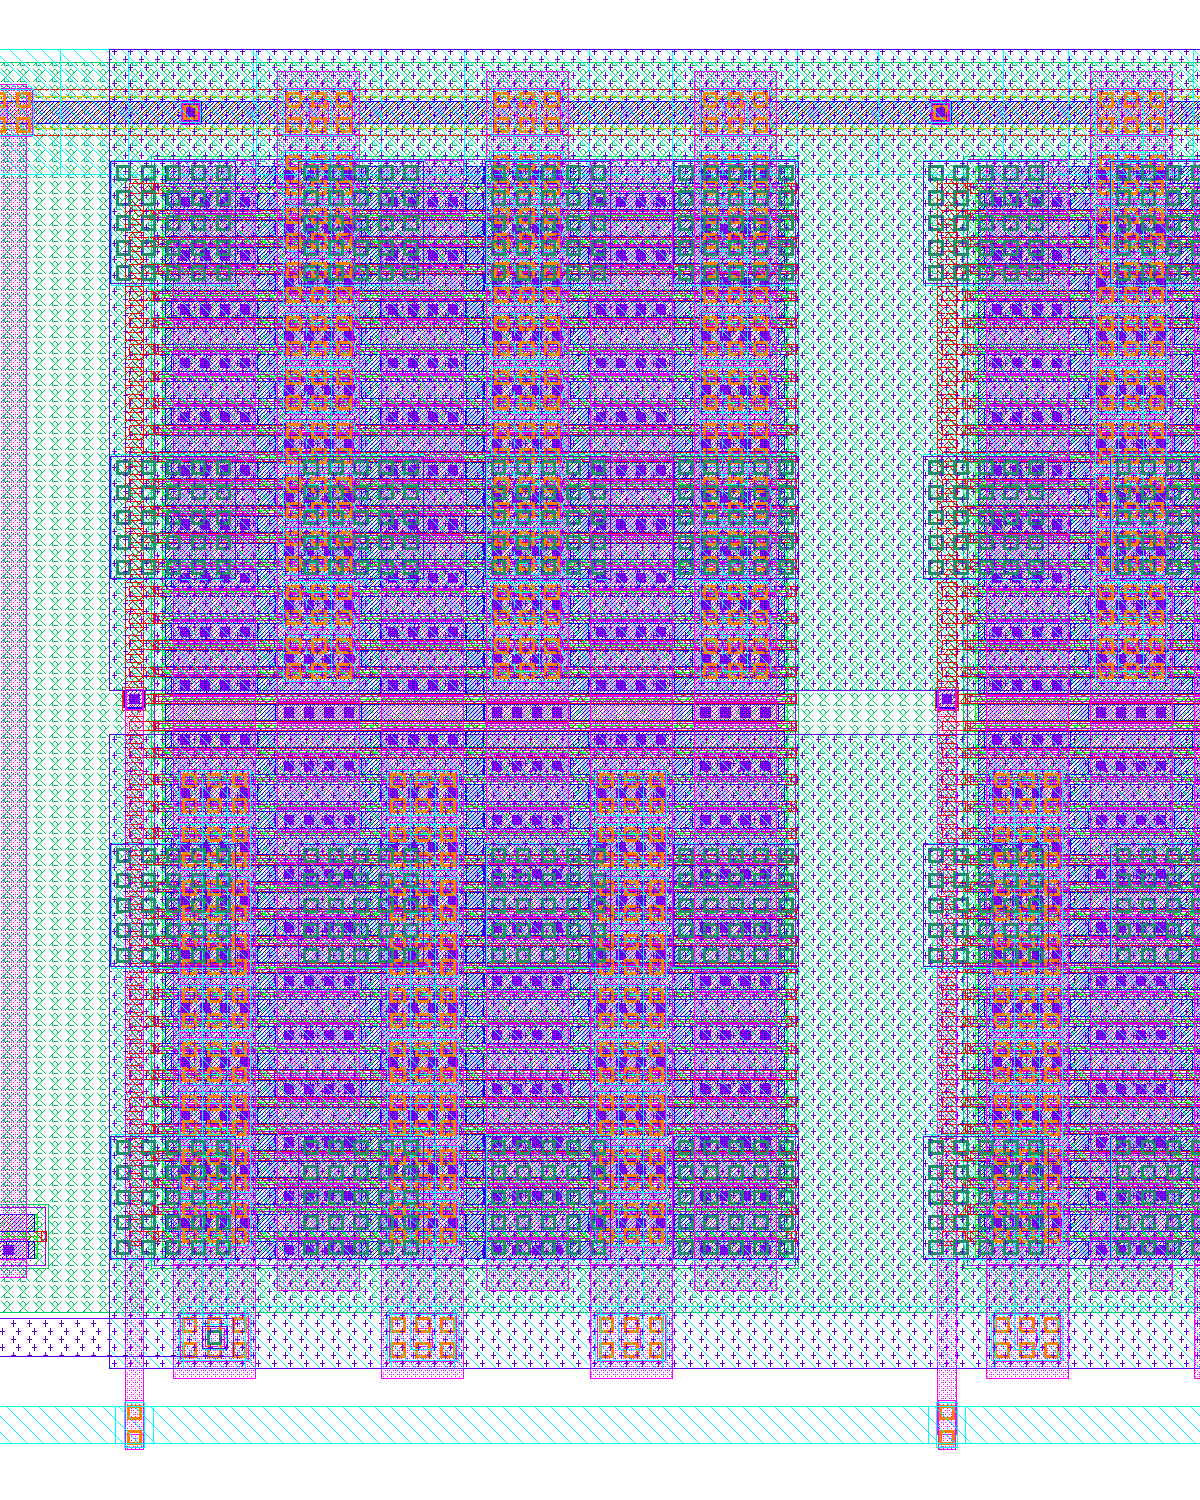
\includegraphics[width=0.48\linewidth]{../figures/layout_pass_zoom.png}
\caption{One pass column and a half: the via2 stacks on the drain straps (lower half, vout plate) and on the source straps (upper half, vin plate), and the via3 arrays.}
\end{figure}

\section{Physical verification}

\subsection{DRC}
Deck: \texttt{sky130A\_mr.drc} (efabless, release 2024.2.11\_01.09), KLayout 0.30.12, front end, back end and off-grid checks. Result on \texttt{ldo\_final.gds}: \textbf{0 violations}. The first run had nine: eight \texttt{licon.1} (the 0.19$\times$2.0\,$\mu$m contact slots of the resistors, exempt only when \texttt{poly\_rs} is present, which Electric had not written) and one \texttt{m3.6} (a 0.16\,$\mu$m$^2$ met3 pad in a via stack, now 0.36\,$\mu$m$^2$). Electric's own DRC still lists errors (psdm spacing between overlapping implant shapes, poly-to-diffusion spacing, and met3 spacing where the plates overlap wires that Electric treats as other nodes); the official deck reports none of them.

\subsection{LVS}
Deck: \texttt{sky130.lvs} (efabless \texttt{sky130\_klayout\_pdk}, commit 13d25721), against a CDL netlist written from \texttt{sizes.json} (\texttt{scripts/ldo\_cdl.py}). Result: \textbf{netlists match}. After the deck combines the fingers and the series resistor units, the extracted netlist is:

\begin{table}[H]
\centering\small
\caption{Devices extracted by the LVS deck (after combining parallel fingers and series units).}
\begin{tabular}{llcc}
\toprule
device & model & $W$ ($\mu$m) & $L$ ($\mu$m) / $R$ \\
\midrule
$M_{BL}$ & pfet\_01v8 & 4 & 1 \\
$M_D$ & pfet\_01v8 & 10 & 0.15 \\
$M_P$ & pfet\_01v8 & 1600 & 0.15 \\
$M_3$ & pfet\_01v8 & 16 & 1 \\
$M_4$ & pfet\_01v8 & 16 & 1 \\
$M_1$ & nfet\_01v8 & 16 & 1 \\
$M_{CS}$ & nfet\_01v8 & 20 & 0.5 \\
$M_2$ & nfet\_01v8 & 16 & 1 \\
$M_T$ & nfet\_01v8 & 16 & 1 \\
$M_{BN}$ & nfet\_01v8 & 4 & 1 \\
$R_1$ & res\_xhigh\_po\_0p35 & 0.35 & $l$ = 8.54\,$\mu$m, 48.8\,k$\Omega$ \\
$R_2$ & res\_xhigh\_po\_0p35 & 0.35 & $l$ = 17.08\,$\mu$m, 97.6\,k$\Omega$ \\
dummies (parallel) & res\_xhigh\_po\_0p35 & 0.7 & $l$ = 4.27\,$\mu$m, 12.2\,k$\Omega$ \\
\bottomrule
\end{tabular}
\end{table}

\noindent To check that the flow can fail, the comparison was repeated with four deliberately wrong netlists (\texttt{layout/lvs\_negative\_test.py}): 150 instead of 160 pass fingers, $M_2$'s gate on $V_{REF}$, one resistor unit 5\,$\mu$m long, $L(M_{CS}) = 0.6\,\mu$m. All four were reported as mismatches, the correct netlist as a match.

\subsection{Electromigration}\label{sec:em}
Limits: the SkyWater technology LEF \texttt{sky130\_fd\_sc\_hd.tlef} (average DC current, junction temperature 90\,\textdegree C): 2.8\,mA/$\mu$m (met1, met2), 6.8\,mA/$\mu$m (met3, met4), and per cut 0.36 (mcon), 0.29 (via), 0.48 (via2, via3)\,mA. The check (\texttt{layout/em\_check.py}) measures widths and cut counts on the GDS and assumes the worst case for each element: the whole current that a branch can carry passes through its narrowest element, with no sharing. At $\IL = 50$\,mA each of the 160 fingers carries 0.31\,mA.

\begin{table}[H]
\centering\small
\caption{EM check of the pass-device path at 50\,mA, worst-case bounds.}
\begin{tabular}{lrrl}
\toprule
element & $I$ (mA) & limit (mA) & measured \\
\midrule
mcon, one S/D row & 0.625 & 9.720 & 27 cuts \\
met1 row bar (all row current, one side) & 0.625 & 0.728 & height 0.26\,$\mu$m \\
via1, one row into one strap (whole row) & 0.625 & 1.160 & 4 cuts \\
met2 strap at the plate edge & 2.292 & 3.668 & width 1.31\,$\mu$m \\
via2 node in vout plate (strap current) & 2.292 & 2.880 & 6 cuts, 30 nodes in column 0 \\
met3 vout plate, full $\IL$ & 50.000 & 63.954 & height 9.40\,$\mu$m \\
met4 vout plate, full $\IL$ & 50.000 & 63.954 & height 9.40\,$\mu$m \\
via3 vout plate (if the pin is met4) & 50.000 & 384.480 & 801 cuts \\
via2 node in vin plate (strap current) & 2.188 & 2.880 & 6 cuts, 33 nodes in column 0 \\
met3 vin plate, full $\IL$ & 50.000 & 64.566 & height 9.50\,$\mu$m \\
met4 vin plate, full $\IL$ & 50.000 & 64.566 & height 9.50\,$\mu$m \\
via3 vin plate (if the pin is met4) & 50.000 & 384.000 & 800 cuts \\
\bottomrule
\end{tabular}
\end{table}

\noindent Every element is within its limit. The closest are the met1 bar of a contact row (0.625 of 0.728\,mA, with all of the row's current assumed to leave on one side) and the plate via2 (2.29 of 2.88\,mA, 2.19 of 2.88\,mA). The limits are for 90\,\textdegree C; at the 125\,\textdegree C corner they are lower, and this was not checked.

\section{Parasitic extraction and post-layout simulation}

\paragraph{Extraction.} KLayout-PEX 0.8.1, 2.5D analytical engine, mode RC, sky130A technology data of the tool. The raw netlist has 34,299 resistors and 64,669 capacitors. ngspice needs about ten minutes for one operating point of it; the netlist was therefore reduced with the TICER pass of the same tool (time-constant threshold 10\,ps, i.e.\ an error per eliminated node of about $2\pi f\tau = 6\times10^{-5}$ at 1\,MHz, exact at DC) to 4,023 resistors and 22,567 capacitors. The full and the reduced netlist give the same operating point ($\VOUT$ = 1.50085\,V, supply current 164.303\,$\mu$A at 0.1\,mA load). The DC sweeps (load and line regulation, dropout, quiescent current) use the same netlist without its capacitors, which do not enter a DC solution; the AC and transient runs use the full reduced RC netlist. The substrate node of the extraction is tied to ground; the 2.5D engine has no substrate resistance. For the loop gain, the gate of $M_2$ is cut from the feedback net in the extracted netlist and the loop is broken there, as in the schematic.

\paragraph{Results.} Table~\ref{tab:summary} compares the two. At light load the two agree closely. At 50\,mA the extracted netlist has a lower loop gain (45.7 against 48.3\,dB) and a \emph{higher} phase margin (101.6\textdegree\ against 80.2\textdegree). The operating point at 50\,mA shows where this comes from (\texttt{scripts/check\_sense\_point.py}): the pass-device drains sit at 1.5095\,V, the top of the divider at 1.4955\,V and the vout pin at 1.4947\,V, i.e.\ 280\,m$\Omega$ of wiring (diffusion, contacts, straps, plate) lies between the drains and the feedback tap and 14\,m$\Omega$ between the tap and the pin. Inserting these two resistors into the schematic raises its phase margin at 50\,mA from 80.2\textdegree\ to 95.5\textdegree\ (unity-gain frequency 1.57\,MHz), so most of the difference is this series resistance. Above about 10\,MHz the post-layout loop gain does not roll off but stays near $-16$\,dB (Fig.~\ref{fig:lg}). This is capacitive coupling into the feedback net, which bypasses the loop break: moving its 224 coupling capacitors (4.8\,fF in total) to ground lowers $|T|$ above 100\,MHz from $-16$ to $-84$\,dB at 0.1\,mA and changes the phase margin at 50\,mA only from 101.6\textdegree\ to 100.1\textdegree\ (\texttt{scripts/check\_fb\_coupling.py}). The remaining 5\textdegree\ were not attributed. (Treating the same resistance as extra ESR of $C_L$ does not reproduce the result: it moves the unity-gain frequency to 25\,MHz, \texttt{scripts/check\_route\_esr.py}.) The same resistance costs $\approx$14\,mV of headroom at 50\,mA, which appears in the post-layout dropout. Phase margin against the ESR of $C_L$ = 0, 10\,m$\Omega$, 1\,$\Omega$, post-layout (schematic in brackets): at 0.1\,mA 89\textdegree\ (89\textdegree), 90\textdegree\ (89\textdegree), 126\textdegree\ (125\textdegree); at 50\,mA 93\textdegree\ (69\textdegree), 102\textdegree\ (80\textdegree), 62\textdegree\ (55\textdegree). The loop stays stable in all of them.

\begin{figure}[H]
\centering
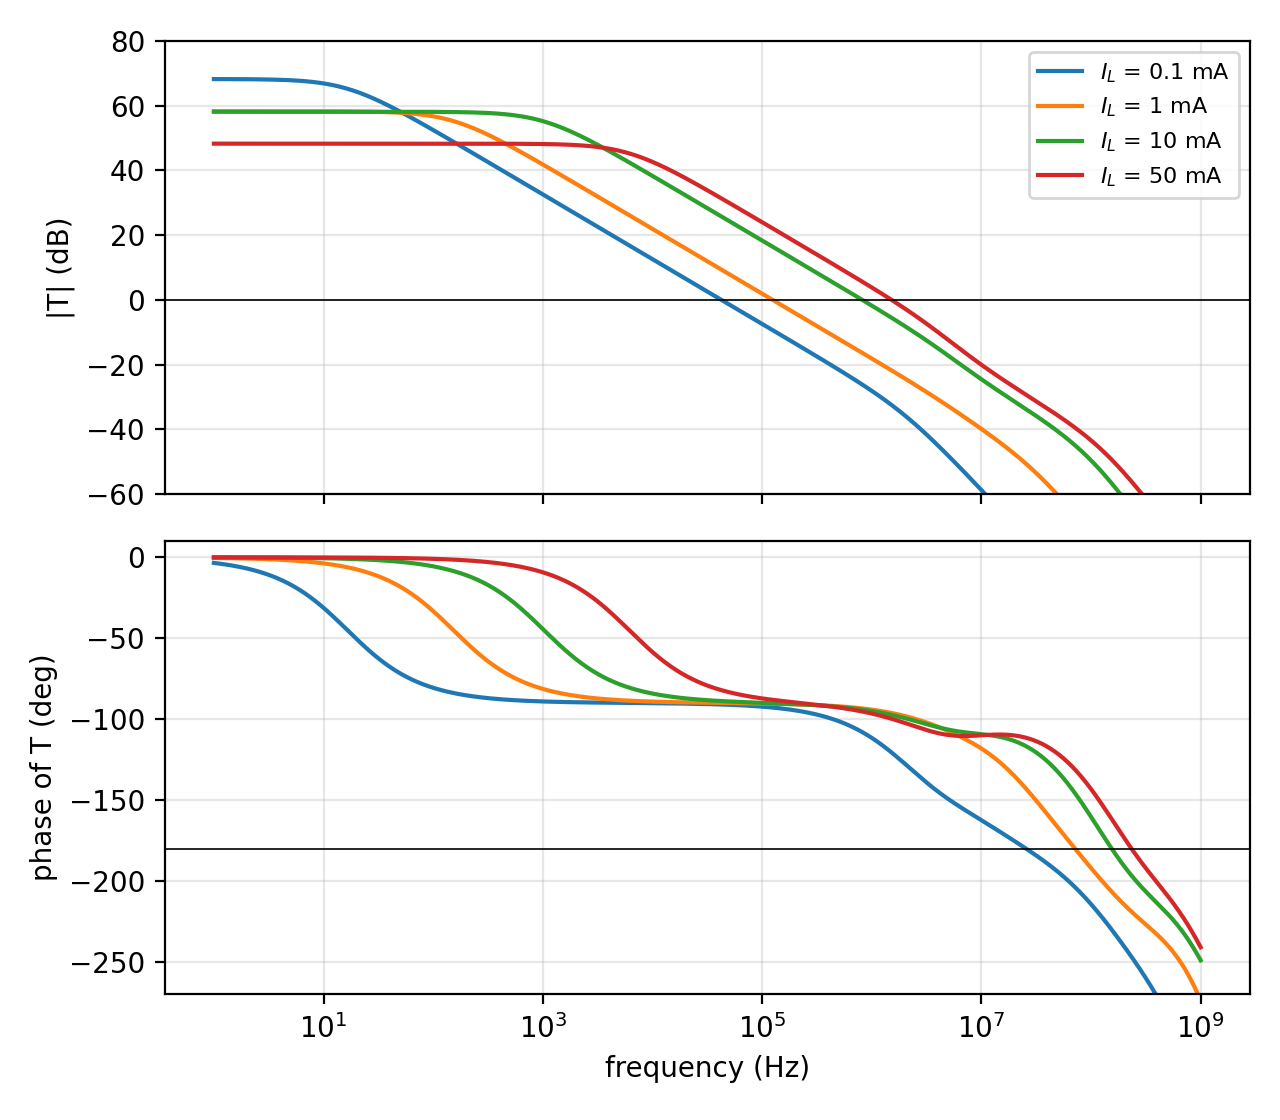
\includegraphics[width=0.49\linewidth]{../figures/loop_gain_sch.png}\hfill
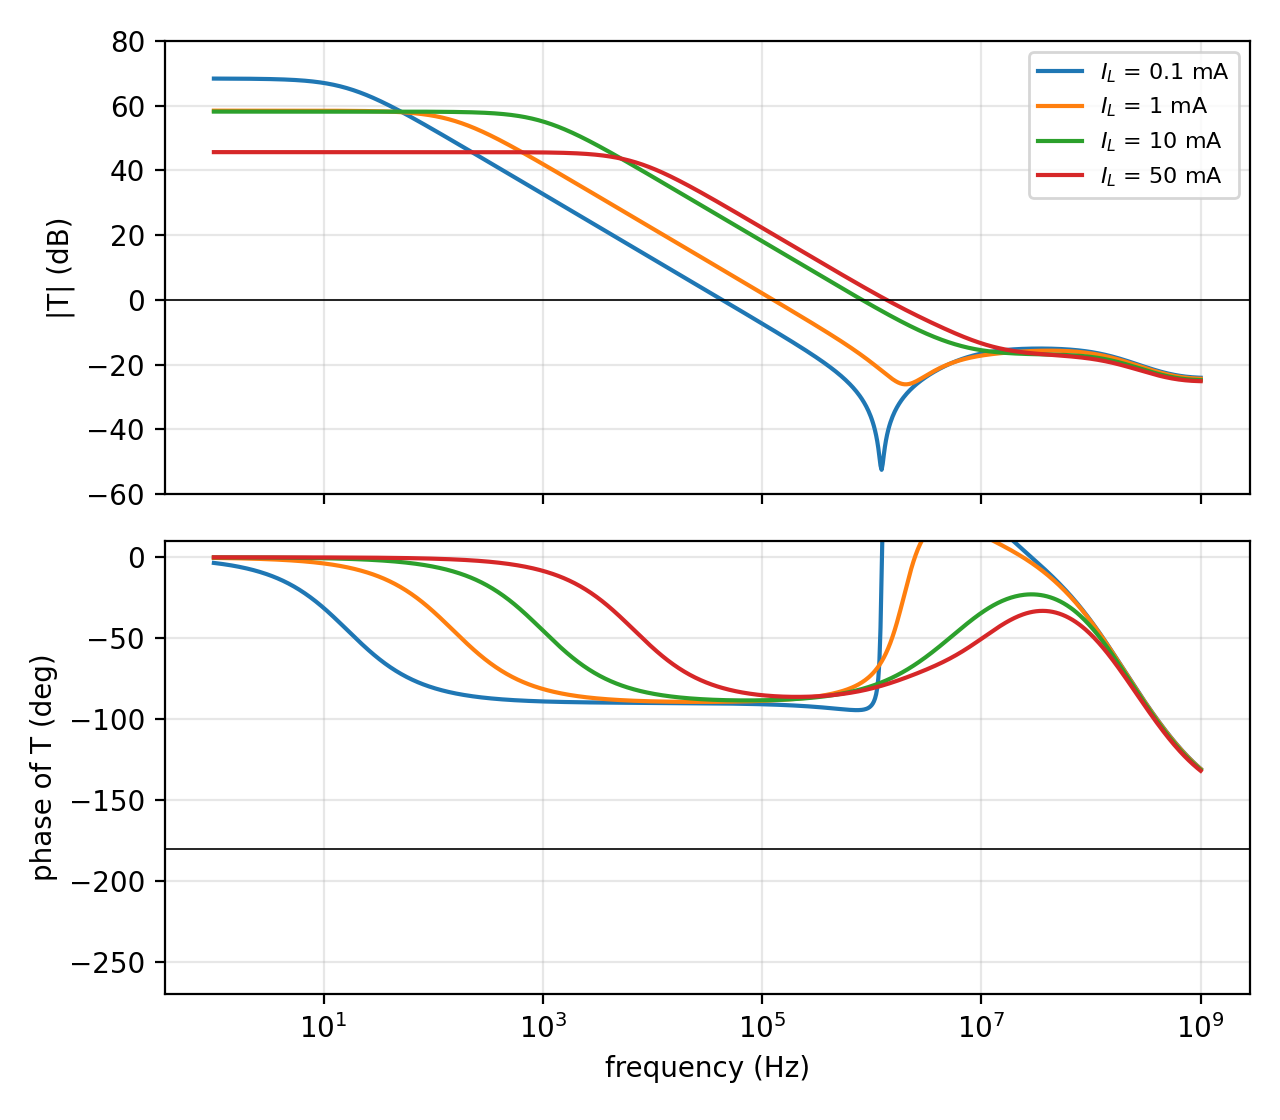
\includegraphics[width=0.49\linewidth]{../figures/loop_gain_pex.png}
\caption{Loop gain, schematic (left) and post-layout (right), at $\IL$ = 0.1, 1, 10, 50\,mA.}\label{fig:lg}
\end{figure}

\begin{figure}[H]
\centering
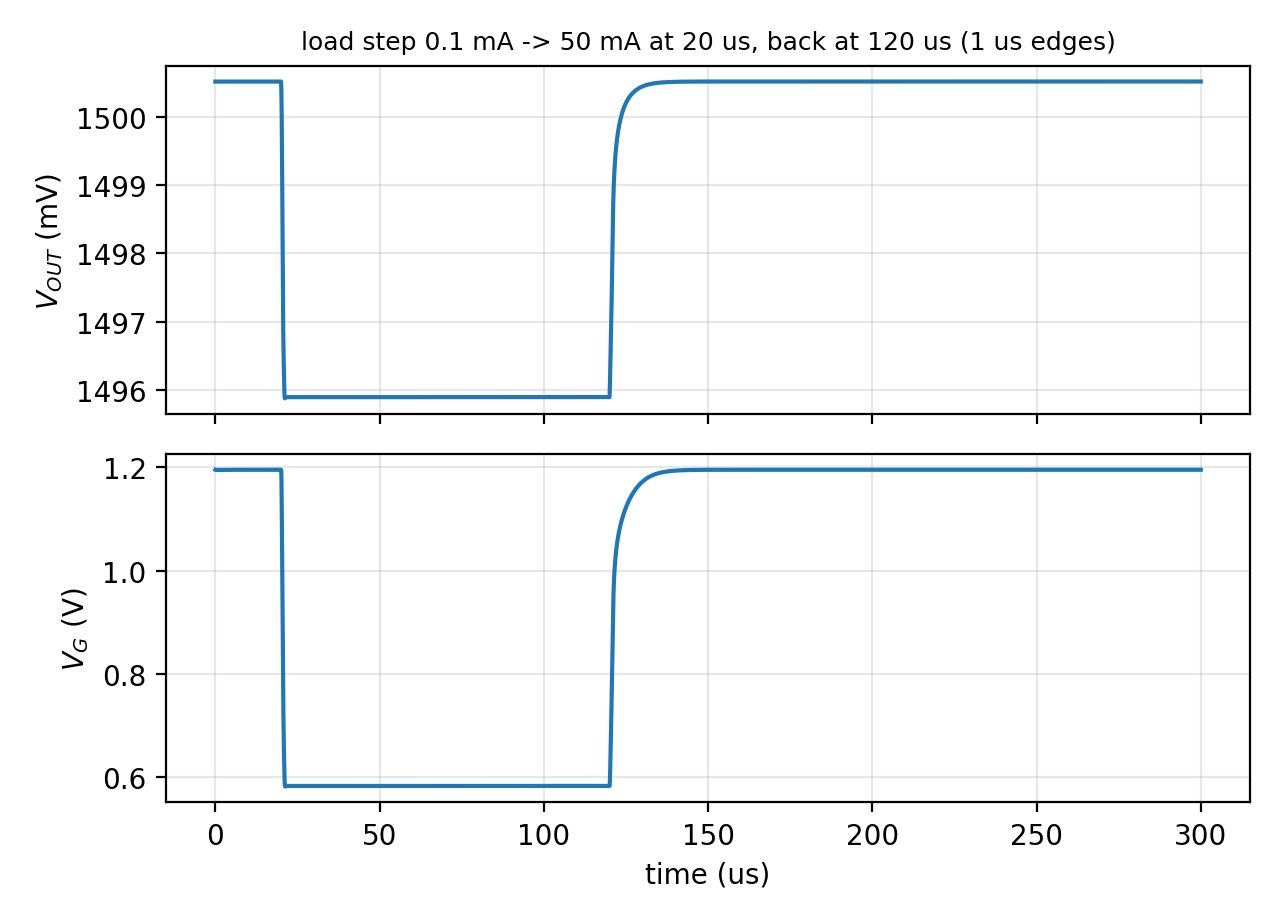
\includegraphics[width=0.49\linewidth]{../figures/load_transient_sch.png}\hfill
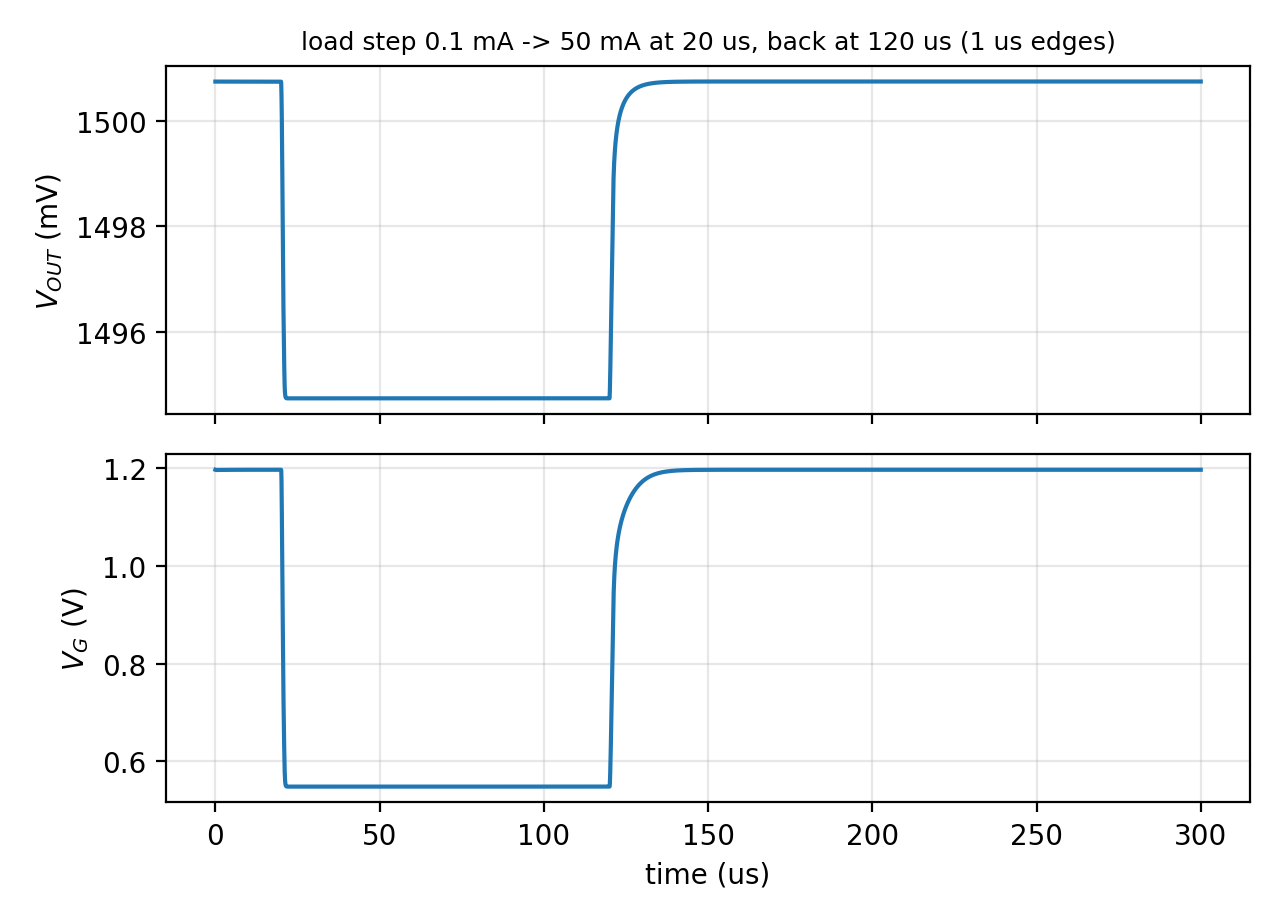
\includegraphics[width=0.49\linewidth]{../figures/load_transient_pex.png}
\caption{Load step 0.1\,mA $\to$ 50\,mA $\to$ 0.1\,mA (1\,$\mu$s edges), schematic (left) and post-layout (right).}
\end{figure}

\section{A numerical artefact in the corner sweep}
The first corner sweep read $\VOUT$ at 50\,mA as the last point of a DC sweep of $\IL$. At hh, 27\,\textdegree C, $\VIN = 1.8$\,V it gave 1.69\,V. The circuit is not at fault: an operating point at 50\,mA and a transient run both give 1.4959\,V, and in the DC sweep 6 of its 500 points jump to non-physical values (one at $-2128$\,V) while the others lie between 1.4959 and 1.5005\,V (\texttt{scripts/check\_hh.py}). The sweep now takes $\VOUT$ from a separate operating point at each load; only this one case changed.

\section{Limitations}
\begin{itemize}
\item The parasitic extraction is the 2.5D analytical engine of one tool; it was not compared with Magic or a field solver, and it has no substrate network.
\item Corners were simulated on the schematic only; post-layout runs are at the typical corner, 27\,\textdegree C, $\VIN = 1.8$\,V. The post-layout ESR sweep has three points (0, 10\,m$\Omega$, 1\,$\Omega$) and the post-layout DC sweeps a coarser step than the schematic ones, because each post-layout AC run takes about five minutes.
\item The block has no pads, ESD, density fill or seal ring; $V_{REF}$ and $I_{BIAS}$ are ideal sources off chip.
\item The pin-and-device-class cross-check of KLayout-PEX did not run (its netlist reader does not accept the three-terminal resistor lines of the CDL file); the connectivity is covered by the LVS deck above.

\end{itemize}

\section{Reproducing}
\begin{verbatim}
cd scripts && python sim_all.py && python corners.py && python check_hh.py
cd ../layout && python gen_layout.py && python run_drc.py && python run_lvs.py
python lvs_negative_test.py && ..\.venv_pex\Scripts\python em_check.py
..\.venv_pex\Scripts\kpex extract --pdk sky130A --gds ldo_final.gds --cell ldo
    --2.5D --mode RC --out-dir pex
python -m klayout_pex.netlist reduce --ticer-tau 10p --ticer-max-degree 8 ...
cd ../scripts && python run_postlayout.py && python check_sense_point.py
cd ../doc && python build_doc.py
\end{verbatim}
\noindent Tools: ngspice 46, Electric 9.08, KLayout 0.30.12, KLayout-PEX 0.8.1, SkyWater sky130 models (\texttt{sky130\_fd\_pr}).

\end{document}
